\documentclass[12pt]{article}
\usepackage[utf8]{inputenc}
\usepackage{titling}
\usepackage{amssymb}
\usepackage{geometry} 
\geometry{a4paper}
\usepackage{graphicx}
\usepackage{hyperref}
\usepackage{wrapfig}
\usepackage{float}
\usepackage{comment}
\usepackage{hyperref}
\usepackage{listings}
\usepackage{tabu}
\usepackage{longtable}
\usepackage{color}
\usepackage[table, svgnames]{xcolor}
\usepackage{array}
\usepackage{cellspace}
\usepackage{minted}

\usepackage[
backend=biber,
sorting=ynt
]{biblatex}
\usepackage{etoolbox}
\addbibresource{my.bib}

\renewcommand*\contentsname{Table of Contents}

\AtBeginEnvironment{tabular}{\rowcolors{1}{\ifnumless{\rownum}{2}{DarkSeaGreen!40}{white}}{}}
\renewcommand{\arraystretch}{2}
 
\begin{document}

\begin{center}

    
\includegraphics[width=6cm]{logo-bath.png} 
    ~\\ 
    ~\\  
    ~\\  
    ~\\ 
    ~\\ 
    ~\\ 
    ~\\ 
    \small Adrian Mircea Nenu
    ~\\ 
    \small Supervisor: Dr. Sheik Meeran
    ~\\ 
    ~\\ 
    \large MSc in Business Analytics
    ~\\ 
    \Huge Stock Clustering and Investment Strategy Optimisation using Dynamic Time Warping Techniques 
    ~\\ 
    ~\\ 
    ~\\    
    ~\\    
    ~\\    
    ~\\    
    \Large April, 2023
    ~\\    
    ~\\    
    \large Submitted as part of the requirement for completing an \\
    MSc in Business Analytics at the University of Bath
    ~\\    
    ~\\    
    \small 13,000 words
\end{center}

\thispagestyle{empty}

\newpage


\begin{center} {\LARGE Abstract} \end{center}

The stock market is a complex and dynamic system, and understanding its underlying patterns is crucial for investment strategy development. Traditional methods for stock analysis, such as linear regression and principal component analysis, can be limited in their ability to capture non-linear relationships and patterns in the data. In this study, we propose the use of dynamic time series warping (DTW) as a powerful tool for stock market analysis. DTW is a non-linear method that allows for the alignment of time series data, even when the time axis is non-uniform. We apply DTW to a data set of historical stock prices and use the resulting similarity matrix to perform clustering. The resulting clusters can be used to identify and analyze similar stocks and inform investment strategy development. 
~\\
We evaluate the performance of our proposed method using several evaluation metrics and compare it with traditional methods. Our results demonstrate that DTW can significantly improve the accuracy and effectiveness of stock market analysis and investment strategy development.

\newpage

\begin{center} {\LARGE Acknowledgements} \end{center}

Firstly, I would like to thank my supervisor, Dr. Sheik Meeran, for his support of the project and for making sure I stayed on track regardless of other competing goals, support thanks to which I have been empowered to manage my time effectively and ensure that I understand all the milestones involved.

Secondly, I would like to thank the professors and professionals who have contributed their ideas and teachings along my journey in this MSc of Business Analytics. 

Last, but not least, I thank my parents and my fiancée for giving me the opportunity to reach my goals, and always cheering me onwards.

\newpage

\tableofcontents

\newpage

\section{Tables and Figures}

\listoftables

\listoffigures

\listoflistings

\newpage

\section{Problem Definition}

\section{Introduction}

\subsection{Overview}

\subsection{Motivations}
Investment strategies and stock clustering can be useful and important for many reasons, amongst which: 

1. Investors use investment strategies to determine which assets to buy or sell, and when to do so, in order to achieve their financial goals. A well-designed investment strategy can help investors navigate market volatility and make informed decisions. 

2. Clustering is the process of grouping similar stocks together based on their characteristics. By identifying clusters of similar stocks, investors can gain insight into patterns and trends in the stock market, which can inform investment decisions. 

3. Diversification: By clustering stocks, investors can identify stocks that are not highly correlated to each other, which can help reduce the risk of a portfolio by diversifying the investments. 

4. Risk management: By identifying clusters of similar stocks, investors can gain a better understanding of the risk associated with different stocks and make more informed investment decisions.

5. Identifying opportunities: Clustering can help investors identify stocks or sectors that may be undervalued or have strong potential for growth, which can lead to investment opportunities.
 
6. Tracking performance: By tracking the performance of stocks within a cluster, investors can identify which stocks are performing well and which are underperforming, which can inform investment decisions. 

\subsection{Data Sets}

\subsubsection{Yahoo Finance}

Stock Prices for companies are obtained through data mining (crawling and scraping) \cite{yahooFinance}.

\subsubsection{S\&P 500}

See in appendices. \pageref{spcode}

\cite{sp500}

\subsubsection{Nasdaq 100}
Used same technique as above plus their API for organization data such as the industry. \cite{nasdaq}

\subsection{Code}

The Github project used in this dissertation serves as a public repository for all of the code and datasets used in the research. The codebase is a combination of Python and JavaScript, and includes both the scripts used to collect and analyze the data, as well as the code used to generate the figures and tables in the dissertation. By making the code and datasets available on Github, the research can be easily replicated and built upon by other researchers in the field. Additionally, it allows for transparency and accountability in the research process.

\url{https://github.com/nenuadrian/msc-business-analytics-dissertation}


\section{Literature Review}

A clustering approach to time series forecasting using neural networks: A comparative study on distance-based vs. feature-based clustering methods. - Manie Tadayon, Yumi Iwashita \cite{ref1}


PATTERNS IN FINANCIAL MARKETS: DYNAMIC TIME WARPING MARIANA, SÁTIRO COELHO  \cite{ref2}


Dynamic Time Warping in Financial Data – Modification of Algorithm in Context of Stock Market Similarity Analysis  \cite{ref3}

A similarity measurement for time series and its application to the stock market - Feng Zhao, Yating Gao, Xinning Li, Zhiyong An, Shiyu Ge, Caiming Zhang  \cite{ref4}


\section{Research Methodology}

\subsection{Overview}

\subsection{Dynamic Time Warping Clustering}

\subsection{Strategy Backtesting}

\section{Analysis and Discussion}

\subsection{Overview}

\subsection{Exploratory Analysis}

asdf asd fasdfasfsadfasf asdfsadf asdfasdfas fasdf asdf
asdf asd fasdfasfsadfasf asdfsadf asdfasdfas fasdf asdf
asdf asd fasdfasfsadfasf asdfsadf asdfasdfas fasdf asdf
asdf asd fasdfasfsadfasf asdfsadf asdfasdfas fasdf asdf

\begin{figure}[H]
\caption{Sample of the stocks data we have gathered.}
\centering
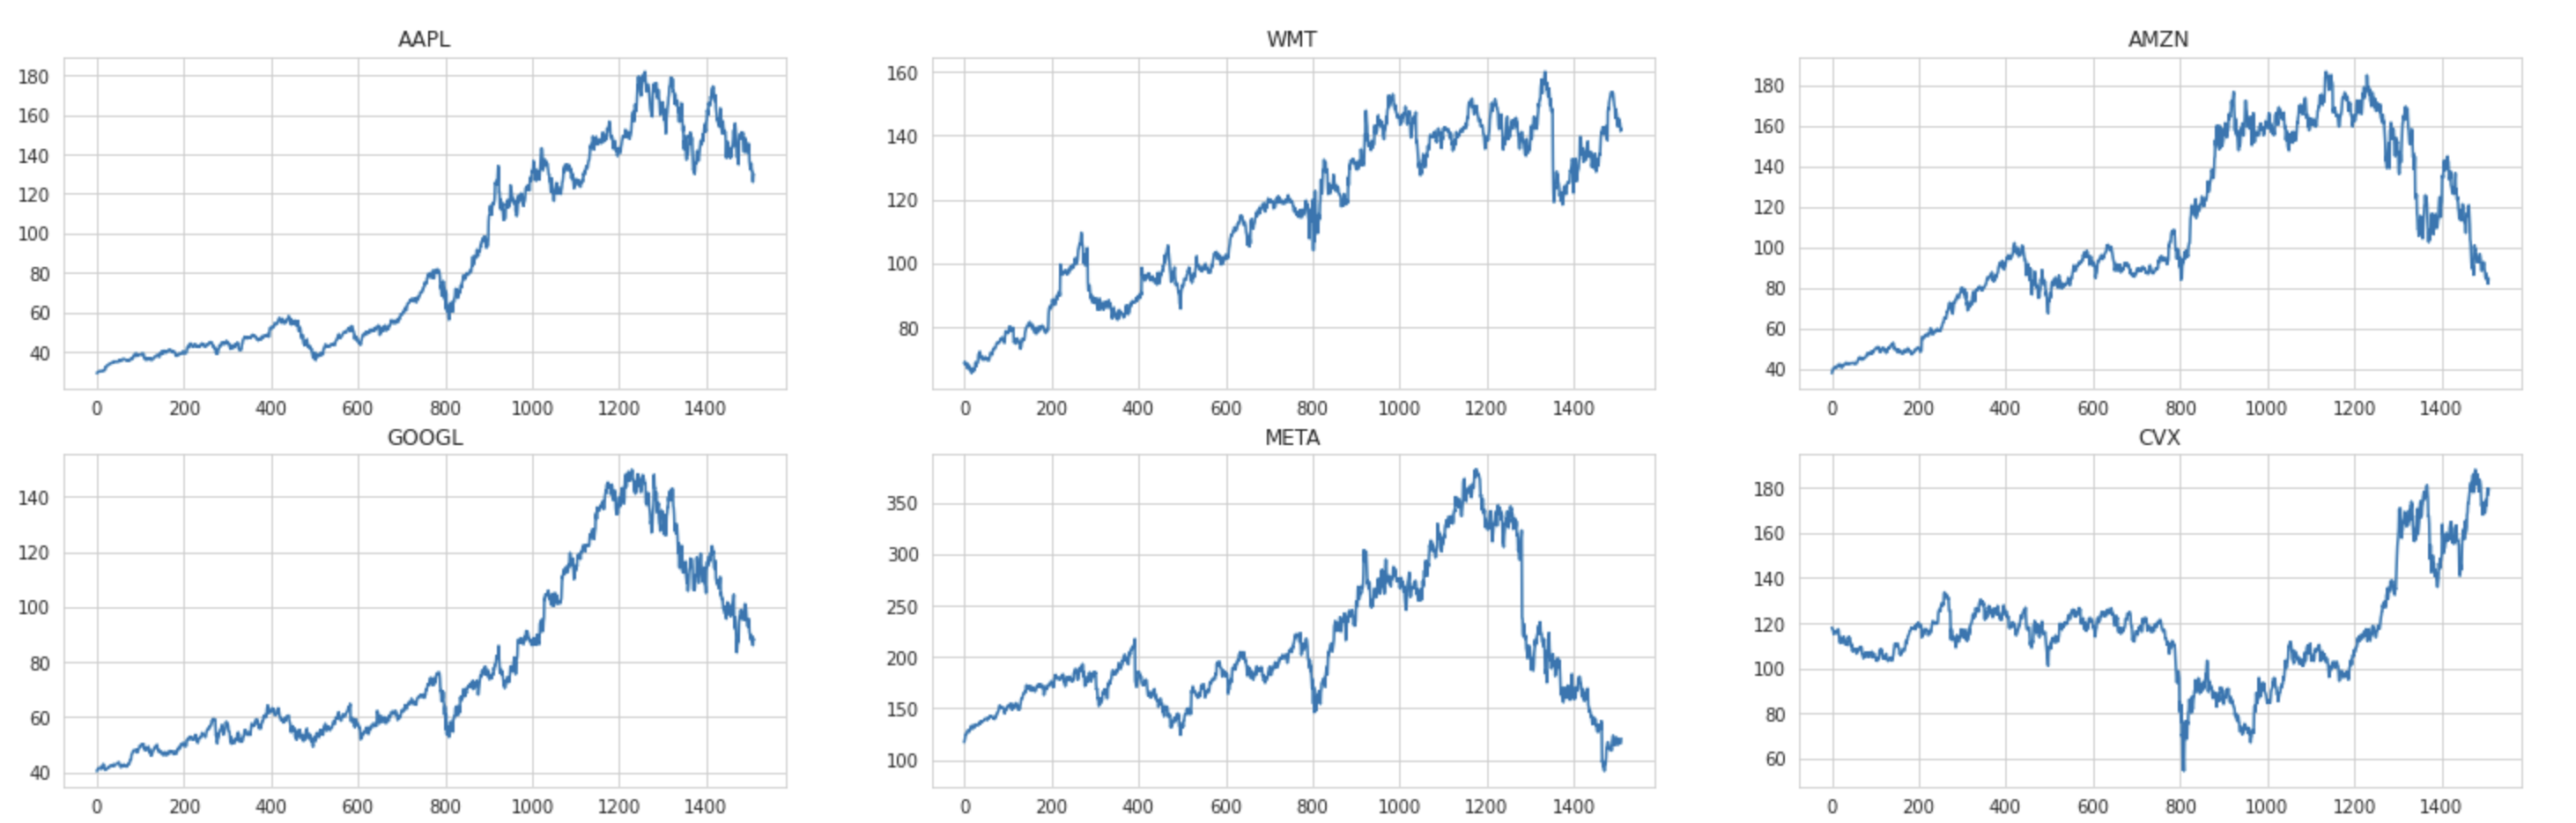
\includegraphics[width=12cm]{img/stocks.png} 
\end{figure}

asdf asd fasdfasfsadfasf asdfsadf asdfasdfas fasdf asdf
asdf asd fasdfasfsadfasf asdfsadf asdfasdfas fasdf asdf
asdf asd fasdfasfsadfasf asdfsadf asdfasdfas fasdf asdf
asdf asd fasdfasfsadfasf asdfsadf asdfasdfas fasdf asdf


\begin{figure}[H]
\caption{Distribution of companies we have gathered data for, by their industry.}
\centering
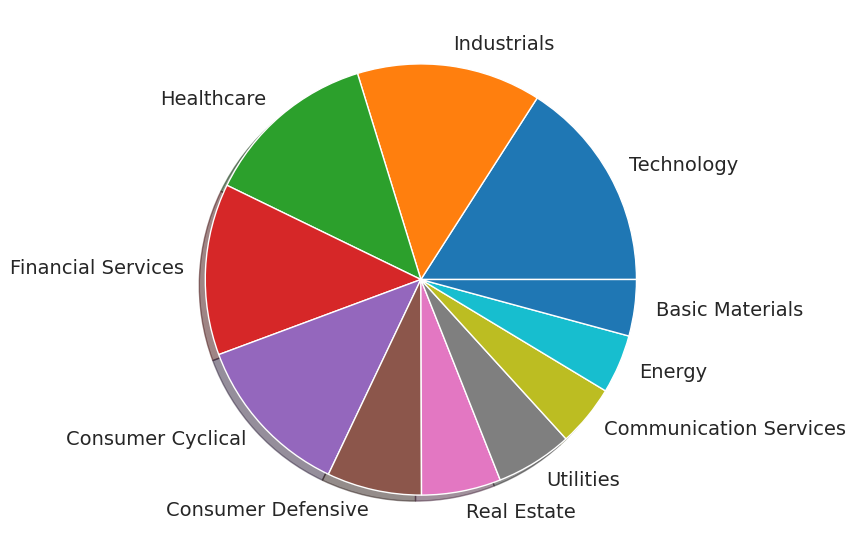
\includegraphics[width=12cm]{img/industries.png} 
\end{figure}


asdf asd fasdfasfsadfasf asdfsadf asdfasdfas fasdf asdf
asdf asd fasdfasfsadfasf asdfsadf asdfasdfas fasdf asdf
asdf asd fasdfasfsadfasf asdfsadf asdfasdfas fasdf asdf
asdf asd fasdfasfsadfasf asdfsadf asdfasdfas fasdf asdf

\subsection{Results of Clustering Techniques}
\subsubsection{MinSom DTW}
\subsubsection{K-Means DTW}

From tslearn \cite{dtwlearn}
\begin{figure}[H]
\caption{DTW Optimization.}
\centering

\[ DTW(x, y) = \min_{\pi} \sqrt{\sum_{(i,j) \in {\pi} }{d(x_i,y_j) }^2} \] 

\[ \pi = [\pi_0,...,\pi_k] \] 


\[ \pi_k = (i_)k,j_k)\ with\ 0 \leqslant i_k < n\ and\ 0 \leqslant j_k < m\]

\[\pi_0 = (0,0)\ and\ \pi_k=(n-1,m-1)\]
\[k>0,\ \pi_k=(i_k,j_k)\ \pi_{k-1}=(i_{k-1},j_{k-1})\]

\[i_{k-1} \leqslant i_k \leqslant i_{k-1} + 1\]
\[j_{k-1} \leqslant j_k \leqslant j_{k-1} + 1\]
\end{figure}



\subsection{Scoring and Comparison}

 
\section{Conclusions}
\subsection{Limitations}
\subsection{Room for Improvement}
\subsection{Concluding Remarks}



\newpage

\section{References}

\printbibliography[title={~}]

\section{Appendices}

\subsection{S\&P Data Extracting Code} \label{spcode}

\begin{verbatim}
const tables = document.getElementsByClassName('table');
Array.from(tables[0].getElementsByTagName('tr'))
    .filter(tr => tr.getElementsByTagName('td')[0])
    .map(tr => { 
        const data = Array.from(tr.getElementsByTagName('td')); 
        return [data[0], data[1], data[2], data[3]]
    .map(td => td.innerText); })
    .map(row => row.join(','))
    .join("\n");
\end{verbatim}

\end{document}
